%----------------------------------------------------------------
%
%  File    :  prediction_model.tex
%
%  Authors : Thomas Lerchbaumer
% 
%  Created :  19 March 2022
% 
%  Changed :  19 March
% 
%----------------------------------------------------------------

\chapter{Predicting Future Bookings}
\label{chap:predict}
The knowledge of potential future bookings provide useful insights when it comes to yield management. Yield management in general describes controlling price and capacity control in a simultaneous ways \cite{yield_m}. Therefore those predictions can be used to support bus operators in their pricing strategy.  This chapter focuses on creating two prediction models utilizing different techniques based on the data that is available. 
Both models are implemented using python and the following libraries. 
\begin{itemize}
\item  \verb|matplotlib|\footnote{https://matplotlib.org/} - used for plotting
\item \verb|pandas|\footnote{https://pandas.pydata.org/} - used for data manipulation 
\item \verb|tesnorflow|\footnote{https://www.tensorflow.org/} - provides ML models
\item \verb|keras|\footnote{https://keras.io/} - Neural Network library
\end{itemize}

As there are various models available a literature review was conducted to figure out which models fit the purpose of time series forecasting. It turns out that the most promising NN that can be utilized for time series prediction are either Convolutional Neural Networks (CNN) or Recurrent Neural Networks (RNN) especially Long Short-Term Memory (LSTM)\cite{nn_1}\cite{nn_2}\cite{lstm_1}\cite{lstm_2}.

\section{Backpropagation}

As both of the models LSTM and CNN use back propagation (BP) for its training the basic concepts of the algorithm are explained in this section. To understand the logic of backpropagation a few terms need a detailed explanation: 
\subsubsection{Gradient}
The gardient also called gradient descent is an algorithm that is used to optimize the loss function within backpropagation. That means that the gradient descent indicates by how much the weights and biases need to be adjusted in order to reduce the actual error value which is the result of the applied loss function. \cite{bp_basic}
\subsubsection{Bias}
The bias is an additional parameter used in each neuron of a NN. It is used to directly influence the activation function to offset the results either to the negative or positive direction. When looking at the sigmoid function without any bias in place where \verb|x| correlates to the input value and \verb|w| indicates the used weight: 
\begin{equation}
 \sigma(x) = \frac{1} {1 + e^{-{(w*x)}}}
\label{eq:eq_4}
\end{equation}
When looking at figure \ref{fig:sig_wo_bias} the weights only influence the steepness of the function but won't shift it along the x axes.
\begin{figure}[H]
	\centering
		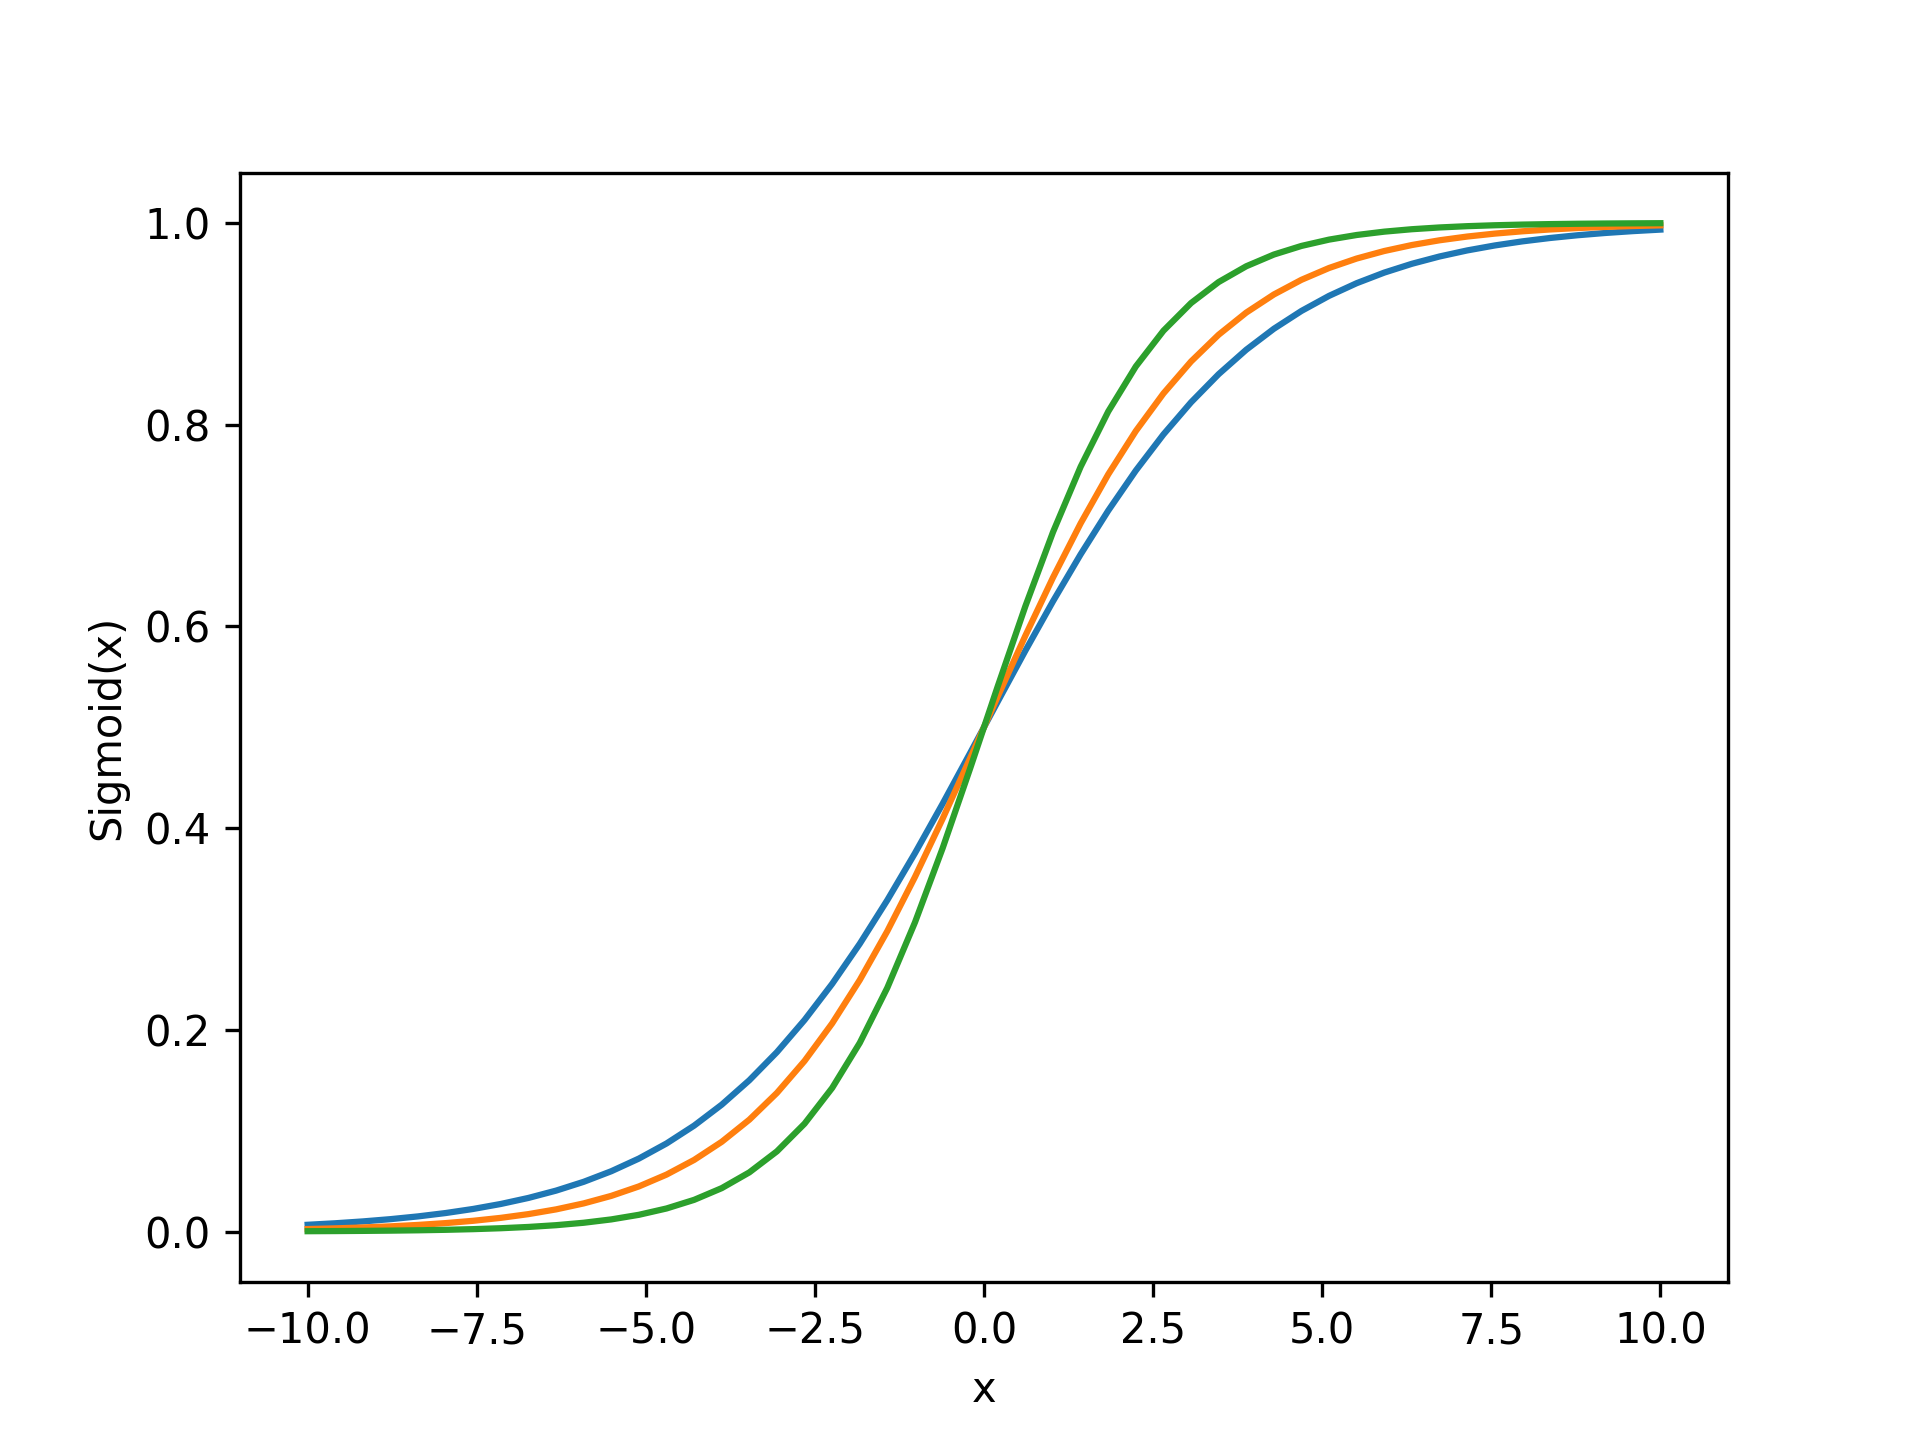
\includegraphics[width=8cm]{images/sigmoid_w_weights}
	\caption{Sigmoid function with different weights and no bias - [source:\cite{lstm_module}]}
	\label{fig:sig_wo_bias}
\end{figure}
 To shift the function along the x axes the sigmoid function is adapted with the bias \verb|b| value: 
\begin{equation}
 \sigma(x) = \frac{1} {1 + e^{-{(w*x+b)}}}
\label{eq:eq_4}
\end{equation}
By adding the bias value as constant to the sigmoid function can be shifted along the x axes as shown in \ref{fig:sig_w_bias}.
\begin{figure}[H]
	\centering
		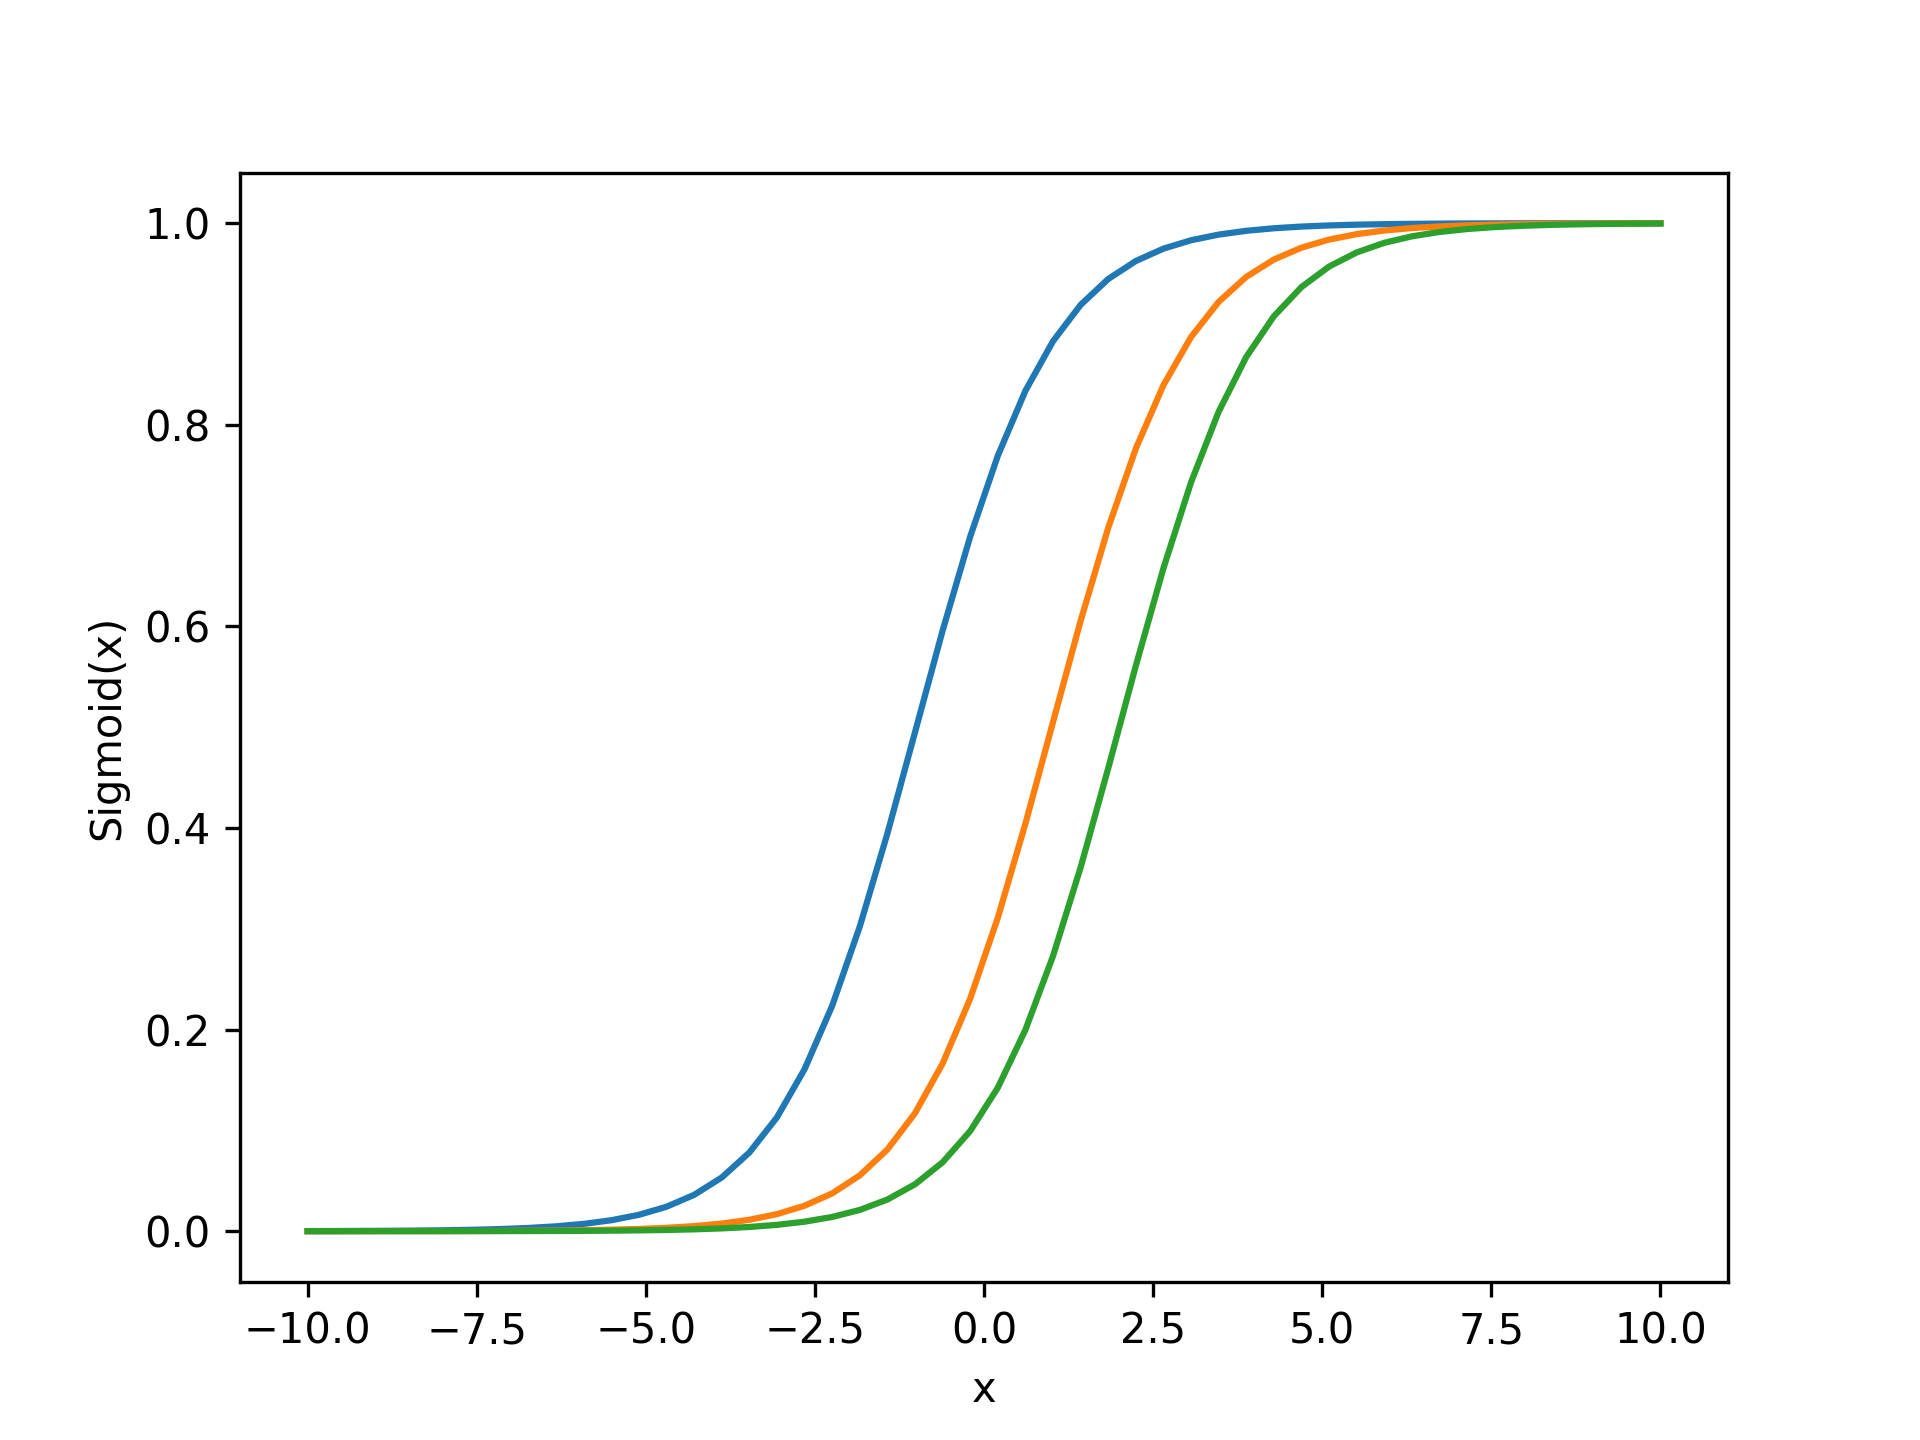
\includegraphics[width=8cm]{images/bias}
	\caption{Sigmoid function with same weights but different bias - [source:author]}
	\label{fig:sig_w_bias}
\end{figure}
The bias therefore is utilized to directly influence the result of the activation function and whether or not a certain neuron is activated or not. 
\subsubsection{Activation Function}
Activation functions introduce non-linearity characteristics to NN. This function is applied to the output of a neuron and decides weather or not a neuron is activated or not.\cite{activation}. In combination with the descent gradient this function enables the NN to learn complex patterns within a training set. Orignially the sigmoid function \cite{bp_basic} was used as activation function for NN but as of today multiple other functions like softmax, Tanh, ReLu emerged \cite{activation}.

\subsubsection{Phases} 
 Backpropagation follows an iterative process. At the beginning there is the feed forward pass. During this phase the input data is passed through all layers. Each hidden layer applies a linear function to create certain weights those outputs then are fed to the activation function. Depending on how many hidden layers are used within the NN the output of the activation function is used as input for the next neuron. At the end the predicted outputs by the model are compared with the actual outputs of the training data. This comparison is evaluated through a loss function. At this step the actual learning process of the model starts by calculating the gradient of the loss function considering the output of the NN. After that the back pass is initiated. Along this phase the gradients of each previous layers are multiplied with a local gradient it's weights which results in a gradient in respect to the layer's inputs. After receiving all gradients  based on the network's input data, all weights and biases are updated and optimized to reduce the result of the loss function. The steps forward pass, loss calculation, back pass, and the updates of weight and biases are repeated to improve the network in an iterative way. \cite{bp_basic} Figure \ref{fig:bp} demonstrates the logic of the backpropagation algorithm. Whereas \verb|wu| represents the updated weights after each iteration.  

\begin{figure}[H]
	\centering
		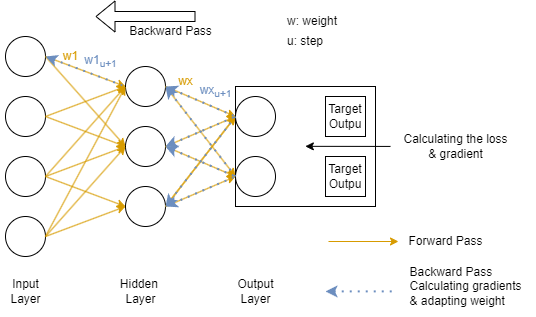
\includegraphics[width=14cm]{images/bp}
	\caption{Simplified logic of the backpropagation algorithmus - [source:\cite{bp_basic}]}
	\label{fig:bp}
\end{figure}
\section{The Models}
Both models CNN and RNN/LSTM can be used for time series forecasting. To create accurate prediction models a basic knowledge about models functionality is required. Therefore this section explains the components of each NN as well as the approaches those models follow. 

\subsection{LSTM}
\label{sec:lstm}
LSTM is an RNN and was invented by \cite{lstm_inventor} in 1997. Until today this NN is widley used for time series forecasting and provides reliable results for short as well as long term predictions \cite{rnn_moharm}. LSTM have so called memory cells which are responsible to store the state of data. Whenever information arrives at a memory cell its outcome is defined by refreshing the cell state with the newly arrived information. LSTM utilizes gates to control a cells state by either including or excluding information \cite{lstm_stock}. The gates are called: 
\begin{itemize}
\item input gate - data selection and storage for upcoming state
\item forget gate - data selection and storage which will not be used for the upcoming state
\item output gate - sets information within the state that is send to the output
\end{itemize}
Those gates are created by combining sigmoid functions. The results of this gates are values ranging from zero to one. A result of zero indicates the cell to not pass any infomration whereas values close to one indicates the cell to pass all information. 
The LSTM Module or Repeating module consists of four NN layers which interact together as shown in Figure \ref{fig:lstm_rep_model}:
\begin{figure}[H]
	\centering
		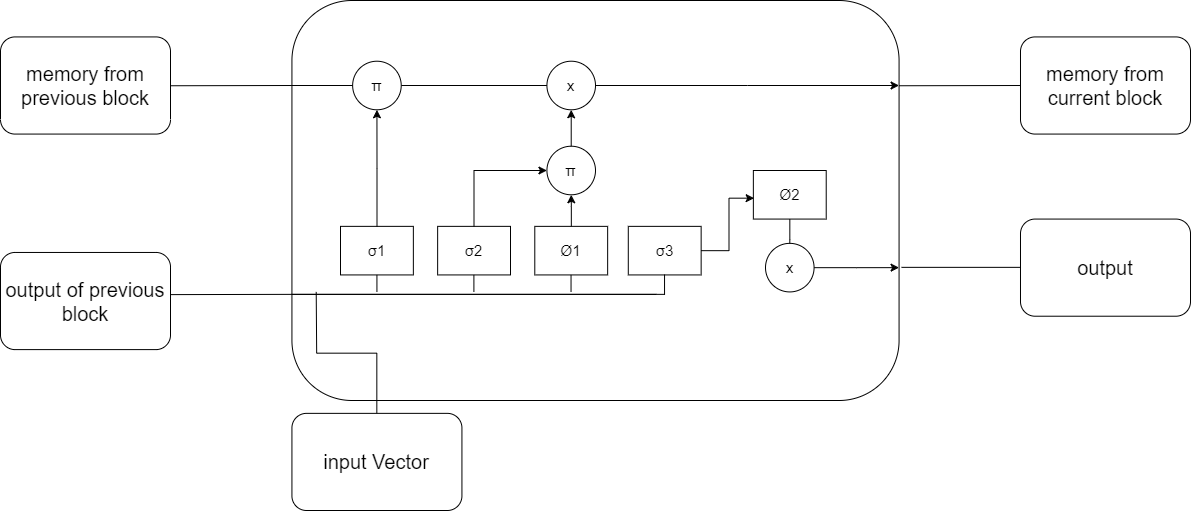
\includegraphics[width=14cm]{images/lstm_module}
	\caption{Repeating LSTM Module - [source:\cite{lstm_module}]}
	\label{fig:lstm_rep_model}
\end{figure}
In total the repeating model has 3 gate activation functions which are named $\sigma_1$, $\sigma_2$,  $\sigma_3$ and shown in figure \ref{fig:lstm_rep_model}. Furthermore $\sigma_1$ and $\sigma_2$ act as output activation functions too. The cell state is illustrated using a blue line which starts at St-1 which indicates the previous memory block to St representing the current memory block. The amount of information that is passed is regulated by layer  $\sigma_1$ using the following function:
\begin{equation}
cf_t = \sigma_1 (W_cf * [O_t-1, x_t] + b_cf)
\cite{lstm_module}
\label{eq:eq_1}
\end{equation}
Furthermore two network layers are used to store new information to the cell state. Therefore sigmoid layer $\sigma_2$ chooses the values which are updated by utilizing the following formula:
\begin{equation}
l_t = \sigma_2(W_1 *[O_t-1, x_t]+ b_l)
\cite{lstm_module}
\label{eq:eq_2}
\end{equation}
Layer $\phi_1$ or \verb|tanh| is created by using new candidate values. This layer outputs a  vector by utilzing the following formular: 
\begin{equation}
\widetilde{S}_t = tanh(W_s * [O_t-1, X_t] + b_s)
\cite{lstm_module}
\label{eq:eq_3}
\end{equation}
The last step includes combination of both states \ref{eq:eq_2} and \ref{eq:eq_3} which is added to the state. Also the state is reconditioned by applying: \cite{lstm_module}
\begin{equation}
S_t = cf_t * S_t1 + I_t * \widetilde{S}_t-1
\cite{lstm_module}
\label{eq:eq_4}
\end{equation}

The reason why a LSTM model is used for this purpose is that a standalone RNN is challenging to train due its characteristics. As Back propagation is used for RNN's problems like vanishing-gradient occur. The gradient in general can be understand as a computed value through all time setps which in the end used to update parameters of the RNN. The vanasihing-gratdient over time results in information decay. By implementing an LSTM module this problem can be solved. \cite{lstm_overcome_rnn_problem}

\subsubsection{Bidirectional LSTM}
Bidirectional LSTMs are able to look in both directions past and future. This is achieved by processing the available data into both directions. Therefore those models make use of bidirectional layers. Those layers split up the used neurons into two directions. \cite{bi_di_1} This provides more information to the network as the model is now capable if storing the forward state as well as the backward state. Resulting in potentially more accurate results \cite{bi_di_2}. 

\subsection{CNN}
\label{sec:cnn}
CNN's follow the concept of NN consisting of multiple layers. The scope of application for this kind of network reaches from computer vision problems to time-series forecast modelling. Whereas data provided for image classification is structured in multi dimensional arrays (matrices), data used for time-series forecasting is provided via one dimensional arrays.\cite{cnn_intro} A CNN provides different types of layers . Those layer types are called pooling layer (PL), fully connected (FC), Convolution layer (CL) and flatten layer (FL). The connection of those layers are demonstrated in figure \ref{fig:cnn_struct}.
\begin{figure}[H]
	\centering
		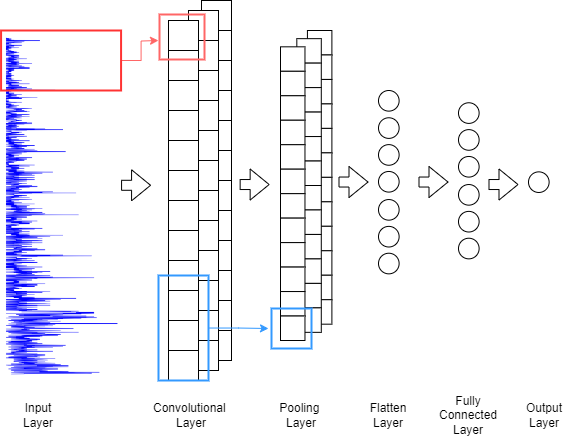
\includegraphics[width=10cm]{images/1d_cnn_model}
	\caption{One Dimensional CNN Structure - [source:\cite{cnn_vechicle}]}
	\label{fig:cnn_struct}
\end{figure}

CNN is based on convolution which is a linear operation that multiplies input data with convolution filters. Those filters which are also called kernels correlate to a set of weights \cite{cnn_vechicle}. The kernel values are created during the learning process and are optimized from the NN utilizing back propagation. Furthermore this layer is utilized to detect features within the given one dimensional array. Those features are stored within a feature map and are calculated by applying convolutions on the input data. One crucial parameter to detect proper features is the size of the kernel. The kernel size can be understand as a number of weights that are multiplied with the input data. After each multiplication the sequence is shifted along the input data. Each shift during this process produces one output which is stored in the feature map. The following example demonstrates how this process is done.\cite{1d_cnn}
\begin{lstlisting}
Input Data: [4,7,10,43,20,10] e.g. number of bookings per day. 
Kernel: [0.5,0.25,0.2] Kernel size = 3
1st Multiplication: 4*0.5 + 7*0.25 + 10*0.2 = 5.75
2nd Multiplication: 7*0.5 + 10*0.25 + 43*0.2 = 14.6
...
Output sequence [5.75, 14.6, ...]
\end{lstlisting}
The second operation that is used within the CNN is called activation function. This non-linear function is utilized to detect complex relationships between variables and are applied onto the feature map. As of today multiple functions like ReLU, Sigmoid and softmax can be used as activation functions \cite{cnn_basic3}.

The pooling layer as shown in figure \ref{fig:cnn_struct} is deployed within a NN to diminish the size of feature maps. To reduce the size pooling operations like average pooling, max pooling or sum pooling can be applied. Applying one of those operations results in less computational efford.\cite{cnn_basic}

The activation function is also part of the fully connected layer. This layer applies the activation function onto the feature map and enables the model in combination with backpropagation to learn complex connections between features. Furthermore this layer operates on the already flatten feature map and outputs a 2d vector.\cite{1d_cnn}

The flatten layer transforms two dimensional input data into one dimensional input vectors. It's output is used to provide outputs to the fully connected layer. Over-fitting can be caused whenever all features are used in the flatten layer therefore a dropout layer can be set in place. This layer cancels out neurons during the training process of a NN which reduces the model's size. 

\section{Overfitting and Underfitting}
One problem that can occur when utilizing NN for predictions is over-fitting or under-fitting of the training data. Both scenarios result in a poor performance of the trained model.
\subsection{Overfitting}

Overfitting describes the phenomenon that the model is not able to improve its problem solving capabilities after a certain period of training. There are multiple reasons for the occurrence of overfitting. One reason for example is a inaccurate or unbalanced training set. This leads to the fact that the NN produces wrong connections during its training.  Whereas the results for the training set are accurate the problems  occur during the validation phase because the model learned wrong characteristics. \cite{fitting} 
\subsection{Underfitting}
On the other hand underfitting arises when the model is not capable of identifying the traits of the training set and therefore struggles to achieve matching its target values. This results in a high loss values. Reasons for underfitting are caused by a lack of trainable parameters as well as a NN model with a simple architecture in terms of hidden layers.
\\\newline In section \ref{sec:data_cleansing} and \ref{sec:data_aug} actions were taken to avoid both overfitting and underfitting. 

\section{Loss Function}
\label{sec:loss_func}
The loss function is one crucial element as they evaluate the accuracy of the produced outputs from a NN. This is achieved by calculating the difference between the predicted value and the actual value provided by the test dataset. Supervised learning deals with two different problems which is either a classification problem i.e. is the animal on the picture a cat or with regression problems which deal with i.e. predicting future bookings. Both of those problems use different loss function.\cite{loss_func} As this section focuses on solving a regression problem a brief overview about available loss functions and their characteristics are given. 

\begin{table*}[htbp]
	\centering
		\begin{tabularx}{\textwidth}{|l|X|}
		\hline
		\rowcolor[gray]{0.9}
		Function & Characteristics \\
		\hline
		Square loss &Sensitive to outliers (Model tends to focus on those outliers whereas accuracy for normal values decline)\\
		 \hline
		Absolute loss & Outliers do not influence the model as severe as compared to square loss  \\
		Huber & Combination of square loss and absolute loss - Outliers do not influence the accuracy of results and learning from smaller errors can still be done in a efficient way  \\
		\hline
		Log-cosh & Similar to Huber when it comes to its characteristics. Does not handle large errors well because the gradient tends to stay constant. \\
		\hline
		Quantile loss & Extends absolute loss and provides prediction intervals. Utilizing a punishment system for overestimated and underestimated samples. \\
		\hline
		$\epsilon$-insensitive & Focuses on samples with large prediction errors \\
		\hline	
		\end{tabularx}
	\caption{Loss functions and their characteristics - [source:\cite{loss_func}]}
	\label{tab:loss_function}
\end{table*}

By looking at the characteristics of the augmented data set shown in figure \ref{fig:augmented_data} it is clear to see that the dataset itself has got outliers repeating themselves every year. To avoid a strong focus on those peaks both models are initial trained utilizing the Adam loss function.

\section{Optimize Function}
\label{sec:optimize_func}
To optimize a NN's parameters an optimizer function is required. This function updates parameters like weights based on the results provided by the loss function \cite{optimizer}. Since both NN's described in this section make use of backpropagation for their training a literature review was conducted to figure out which optimizer is keen to deliver the most accurate results. By inspecting the advantages and disadvantages proposed by these works \cite{optimizer}\cite{optimizer_1}\cite{optimizer_2} it turns out that the algorithm ADAM is a valid choice. This algorithm is characterized by achieving faster convergence compared to other algorithms. Furthermore Adam provides a decent performance for datasets with meager features.

\section{Implementation}
\label{sec:implementation}
Both models follow the same workflow when it comes to their implementation. The workflow is highlighted in figure \ref{fig:workflow}:

\begin{figure}[H]
	\centering
		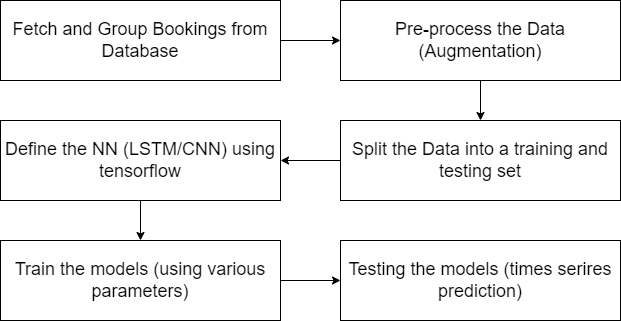
\includegraphics[width=8cm]{images/workflow_imp}
	\caption{Workflow of the implementation - [source:[author]]}
	\label{fig:workflow}
\end{figure}

As each booking correlates to one entry within the database table the data those entries need to be grouped on a daily basis. Therefore the following sql query is executed: 
\begin{lstlisting}
import mysql.connector
import logging
import pandas as pd

def get_booking_data():

       sql = ("SELECT count(taskFrom_time) as bookings, date(taskFrom_time) "
           "from bookings_2 "
           "WHERE date(taskFrom_time) <= DATE('2023-05-01') and date(taskFrom_time) >= 			DATE('2017-01-01') "
           "Group By date(taskFrom_time) order by date(taskFrom_time) asc")

    res = pd.read_sql(sql, connection)
    return res
\end{lstlisting}

Once the data is retrieved from the database it is directly converted to a \verb|pandas dataframe|. As mentioned in chapter \ref{sec:data_aug} data augmentation is necessary to compensate the lack of data during COVID19 \ref{sec:data_aug}. Corresponding to the workflow described in figure \ref{fig:workflow} the data now needs to be separated into a training and test set. The training set is used to train the model whereas the test set is used to display how the trained model performs. Therefore the trained model is used to predict the values for timestamps used in the test set. By reviewing other scientific works that deal with time series forecasting \cite{1d_cnn},\cite{cnn_vechicle},\cite{cnn_intro},\cite{lstm_overcome_rnn_problem},\cite{lstm_module},\cite{lstm_stock} the most accurate results are achieved by using ranges from 80\% to 90\% for training and depending on the range for training data a range of 20\% to 10\% for test data are recommended. The initial split used for both models correlates to 90\% training data to 10\% test data as visualized in \ref{fig:training_test} . Therefore the following code is applied to split the data:
\begin{lstlisting}
training_end = pd.to_datetime('2022-10-31')
#total range 2017-01-01 - 2023-05-31 = 2342 days
train = df[:training_end]
# 2017-01-01 - 2022-10-31 = 2129 days ~ 90%
test = df[training_end:]
# 2022-10-31 - 2023-05-01 = 213 days ~ 10%
\end{lstlisting}
\begin{figure}[H]
	\centering
		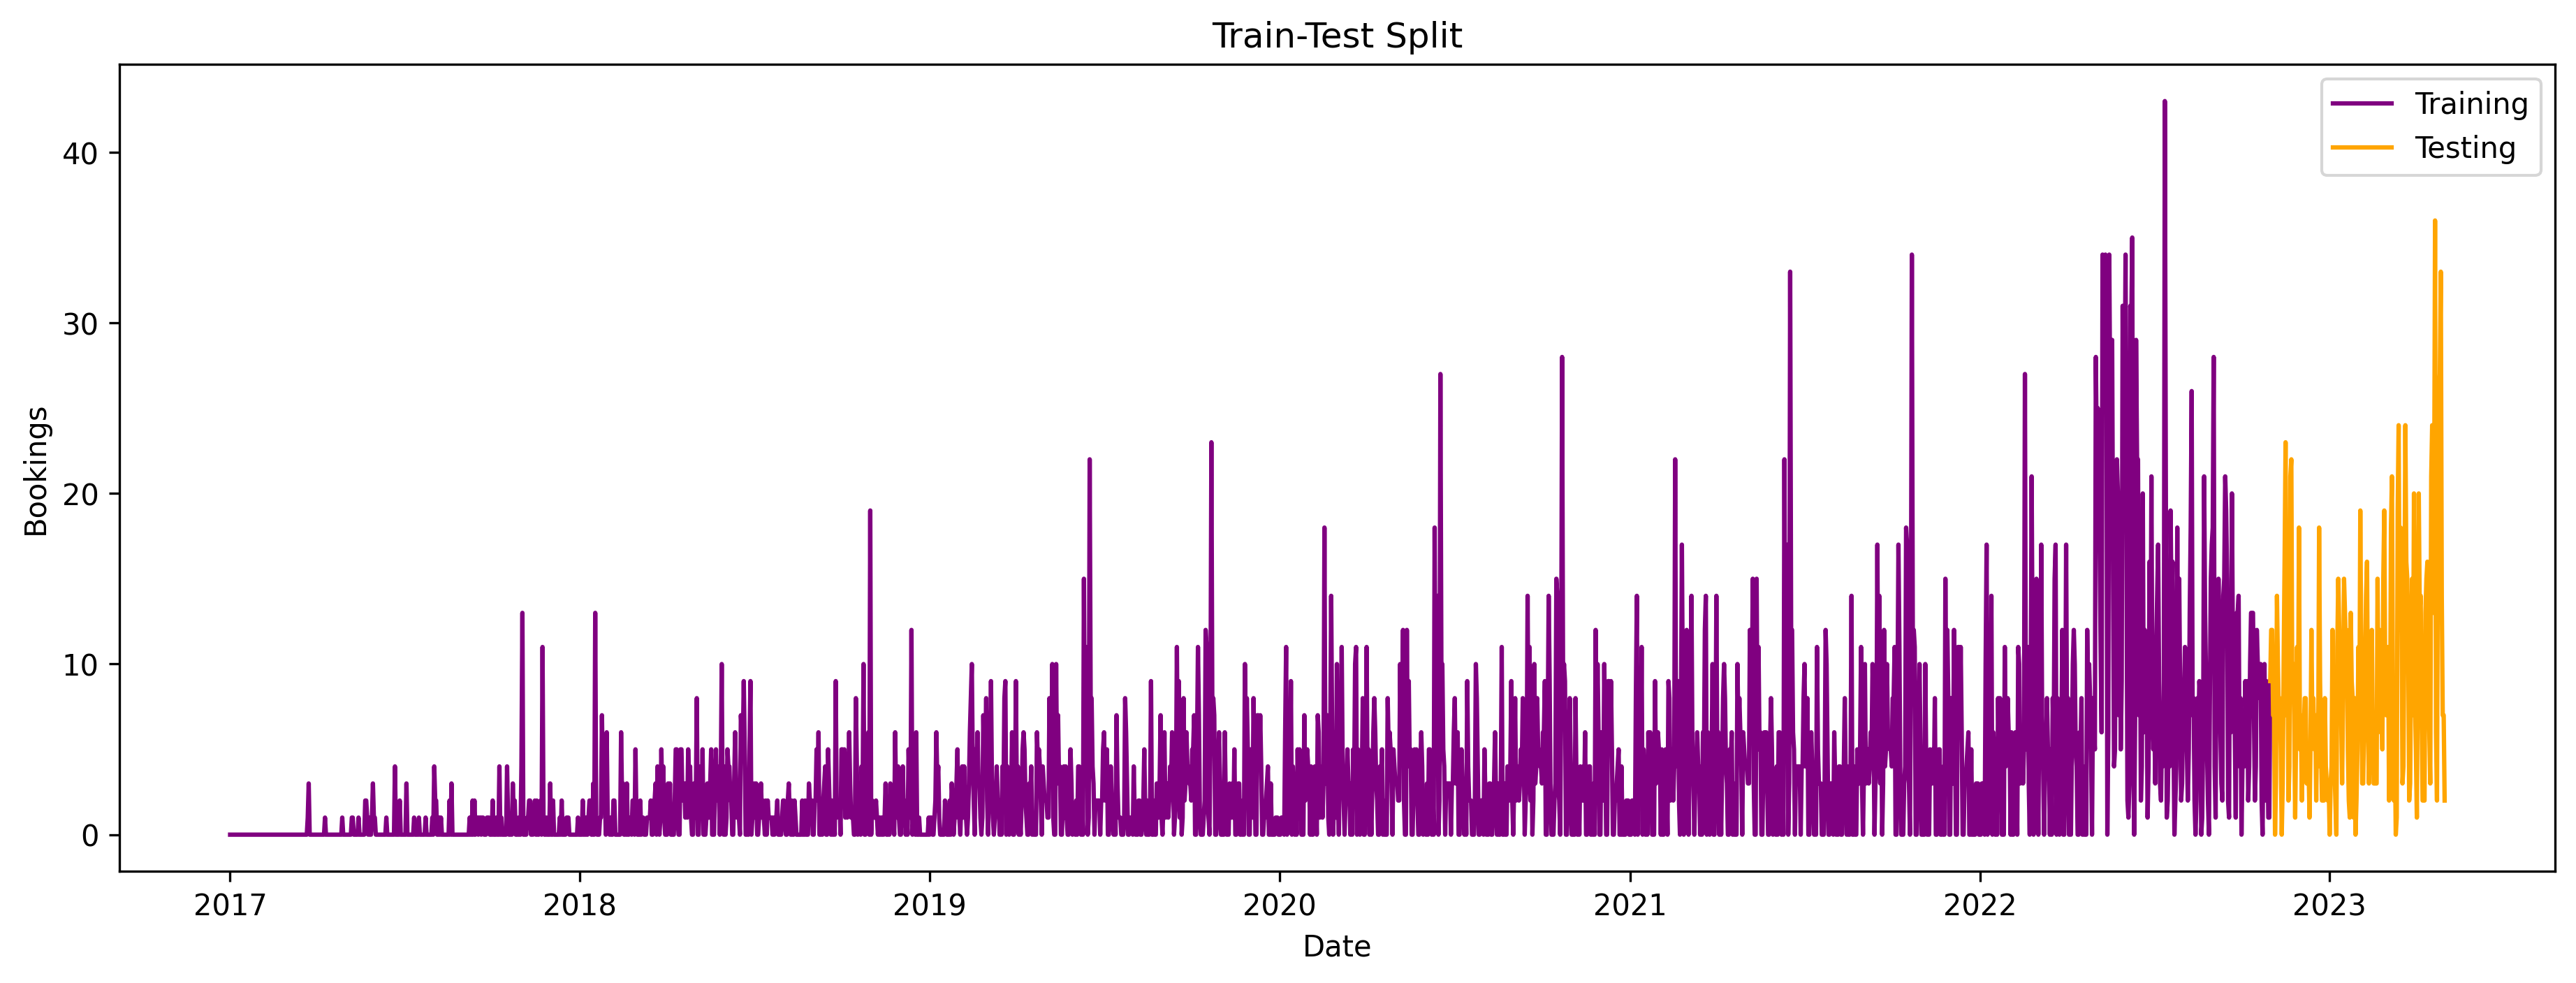
\includegraphics[width=14cm]{images/training_test}
	\caption{Visualized Training-Test split (90\%-10\%) - [source:[author]]}
	\label{fig:training_test}
\end{figure}
With the training and test data in place the next step is to implement both models (LSTM, CNN) by utilizing the \verb|tensorflow| library. To reduce computation costs and to increase training efficiency the training data is further processed.
\begin{lstlisting}
WINDOW = 20
bookings_training_90 = tf.data.Dataset.from_tensor_slices(train.values)
bookings_training_90 = bookings_training_90.window(WINDOW + 1, shift=1, drop_remainder=True)
bookings_training_90 = bookings_training_90.flat_map(lambda x: x.batch(WINDOW + 1))
bookings_training_90 = bookings_training_90.map(lambda x: (x[:-1], x[-1]))
\end{lstlisting}
On line 2 the code above transforms the training data into a \verb|TensorSliceDataset|. This data format grants access to tensorflows data API which supports the user to manipulate the data further. As this is time serires data the model itself is fed with data limited to certain ranges. The constant \verb|WINDOW| indicates a range of 20 days which is used for training. The function \verb|flat.map()| is now used to flatten the dataset. As \verb|from_tensor_slices()| creates a single tensor for each entry in a window \verb|flat.map()| combines those windows to a single tensor holding the windowed data. Line 5 prepares the data and splits each window into features and target values. As the learning process described in section \ref{chap:Backpropagation} involves multiple inputs that are used to predict one output the \verb|.map()| function prepares each windowed tensor by using the interval from \verb|x to x-1| to predict \verb|x-1|.
Both models LSTM and CNN are trained with the prepared data explained in during this section. 

\subsection{Implementation of LSTM}
The code itself required to setup a LSTM model only requires a few input parameters. Therefore it is crucial to understand the meaning behind the input parameters as well as how they can influence the training results of the model itself. The following code is used to initialize the model:   
\begin{lstlisting}
#define the model
lstm_booking_prediction_model = Sequential([
    Lambda(lambda x: tf.expand_dims(x, axis=-1), input_shape=[WINDOW]),
    Bidirectional(LSTM(128, activation='tanh',recurrent_activation='sigmoid' )),
    Dense(units=128, activation='relu'),
    Dropout(0.4),
    Dense(1)
	])
\end{lstlisting}
When utilizing LSTM for time series predictions a certain input format for data is needed. Therefore the Lambda function on line 3 is required to reshape the dimension of the used input data. 
\verb|Bidirectional()|\footnote{\label{tf_fn}\url{https://www.tensorflow.org/api_docs/python/tf/keras/}} actually represents a wrapper for the actual layer used for this model. In this case its holding additional states and is used to created a Bi-LSTM model as described in \ref{sec:lstm}. \newline
\verb|LSTM()|\textsuperscript{\ref{tf_fn}} contains the logic actual logic as described in \ref{sec:lstm}. Furthermore the parameter \verb|unit=128|\textsuperscript{\ref{tf_fn}} can be understand as the number of neurons used within this layer. Furthermore this model offers different kind of activation functions. By default the hyperbolic tangent (tanh)\cite{tanh} is used. Whereas the \verb|recurrent_activation| defines which functions are used for the actual gates within the module as described in \ref{sec:lstm}. Whenever creating a stacked LSTM model, which means it makes use of at least two LSTM layers the paramater \verb|return_sequences| must be set to true. Otherwise the layer's output results in a 2D tensor output which only provides information about the last timestep. This format cannot be passed on to the next LSTM layer. \newline
\verb|Dense()| is used to implement fully connected layers whereas \verb|units| correlate to the amount of neurons used for this layer The last \verb|dense(1)| layer is used to reduce the number of outputs to 1. The way this layer works is explained in section \ref{sec:cnn}. Additional the model needs to be compiled. Therefore the following code is required: 
\begin{lstlisting}
#compile the model 
lstm_booking_prediction_model.compile(
    loss=Huber(),
    optimizer=Adam(),
    metrics=['mae']
	)
\end{lstlisting}
The Parameter \verb|loss| sets the loss function which is utilized to evaluate the models performance. The reason why \verb|Huber| is used is explained in section \ref{sec:loss_func}. Futhermore the model also requires an optimizing algorithm. This algorithm is assigned by using the \verb|optimizer| parameter. Due to the results of a literature review explained in section \ref{sec:optimize_func} Adam turned out to be the most promising candidate for this purpose. To observe the capability of learning of a given model the metric mean absolute error(mea) can be used. 

The next step is to start the training of the model as demonstrated below:
\begin{lstlisting}
#start to train the model
lstm_history = lstm_booking_prediction_model.fit(
    bookings_training_90,
    epochs=100,
    verbose=1,
    use_multiprocessing=True
	)
\end{lstlisting}
The function \verb|fit()| requires parameters like the data used for training (\verb|bookings_training_90|) as well as how many epochs are processed. One \verb|epoch| covers the process of iterating through the entire training dataset and performing forward and backward propagation as well as updating the model's parameters based on the chosen optimization algorithm.
\newline
When training the model using the initial parameters described during this chapter the following results are achieved:



\subsection{Implementation of CNN}
Similar to the implementation of LSTM the implementation of a CNN does not require much code. Furthermore some parts of the code use the same parameters. Those parameters are not explained again. To initialize a CNN model the following code is required: 

 \begin{lstlisting}
#define the model 
cnn_model = Sequential([
    Lambda(lambda x: tf.expand_dims(x, axis=-1), input_shape=[WINDOW]),
    Conv1D(filters=512, kernel_size=3, activation='relu'),
    Conv1D(filters=512, kernel_size=3, activation='relu'),
    GlobalAveragePooling1D(),
    Flatten(),
    Dropout(0.3),
    Dense(512, activation='relu'),
    Dropout(0.4),
    Dense(1)
])
\end{lstlisting}
\verb|Conv1D()| is used to add one one dimensional CL to the model. Those Layers work as described in \ref{sec:cnn}.  The \verb|filter| parameter is equivalent to the number of neurons this layer is going to use. Furthermore the kernel's size as explained in \ref{sec:cnn} is determined by the parameter \verb|kernel_size|.
The only difference left in comparison to the LSTM layer is the FL \ref{sec:cnn}. This layer is added by utilizing the \verb|Flatten()| parameter. When it comes to compiling and fitting the model the CNN makes use of  \verb|Huber()| for its loss function and \verb|Adam()| for its optimization function contrary to the implementation of the LSTM model. Furthermore both models are initially using 100 epochs for their first training. \newline

The first training results produced by the CNN model look the following: 



\section{Reliability Comparison - LSTM, CNN}

\section{Model accuracy}
Having a look at the model performance accuracy (comparing predictions of the model with already available data) , explain potential twerks that have been applied to the model itself to achieve a higher level of accuracy.

